\documentclass[10pt,a4paper]{article}
\usepackage[utf8]{inputenc}
\usepackage[margin=0.6in]{geometry}
\usepackage{graphicx}
\usepackage{microtype}
\usepackage{titlesec}
\usepackage{hyperref}
\usepackage{booktabs}
\usepackage{enumitem}
\usepackage{xcolor}
\usepackage{tabularx}

\graphicspath{{certificates/}{./}}

\definecolor{amritablue}{RGB}{0, 51, 102}
\definecolor{darkgray}{RGB}{50, 50, 50}

\hypersetup{
    colorlinks=true,
    linkcolor=amritablue,
    urlcolor=amritablue,
}

\titlespacing*{\section}{0pt}{4pt}{2pt}
\titlespacing*{\subsection}{0pt}{3pt}{1pt}

\titleformat{\section}
  {\normalfont\small\bfseries\color{amritablue}\uppercase}
  {\thesection}{1em}{}[\titlerule]

\setlist{nosep, leftmargin=13pt}

\begin{document}
\pagestyle{empty}

% =========================================================
% PAGE 1: COURSE COMPLETION CERTIFICATE
% =========================================================
\begin{center}
    {\large\textbf{\color{amritablue}AMRITA VISHWA VIDYAPEETHAM}}\\[1pt]
    {\footnotesize\textbf{Amrita School of Computing, Coimbatore --- Department of Computer Science and Engineering}}\\[2pt]
    {\footnotesize\textbf{Technical Enrichment Activity: Professional Online Certification (20 Marks)}}\\[1pt]
    {\scriptsize Official Course Completion Certificate}
\end{center}

\vspace{-4pt}
\hrule height 0.8pt
\vspace{6pt}

\noindent
\begin{tabularx}{\textwidth}{@{}l X l X@{}}
    \textbf{Student Name:} & Nishanth K & \textbf{Course Title:} & Implementing Security in IoT and Edge Devices \\
    \textbf{Roll Number:} & CB.SC.U4CSE23523 & \textbf{Platform / Provider:} & Coursera / LearnQuest \\
    \textbf{Degree \& Branch:} & B.Tech CSE (VII Semester) & \textbf{Project Guide:} & Ms. Neethu M R (Asst. Professor) \\
\end{tabularx}

\vspace{12pt}
\begin{center}
    \fbox{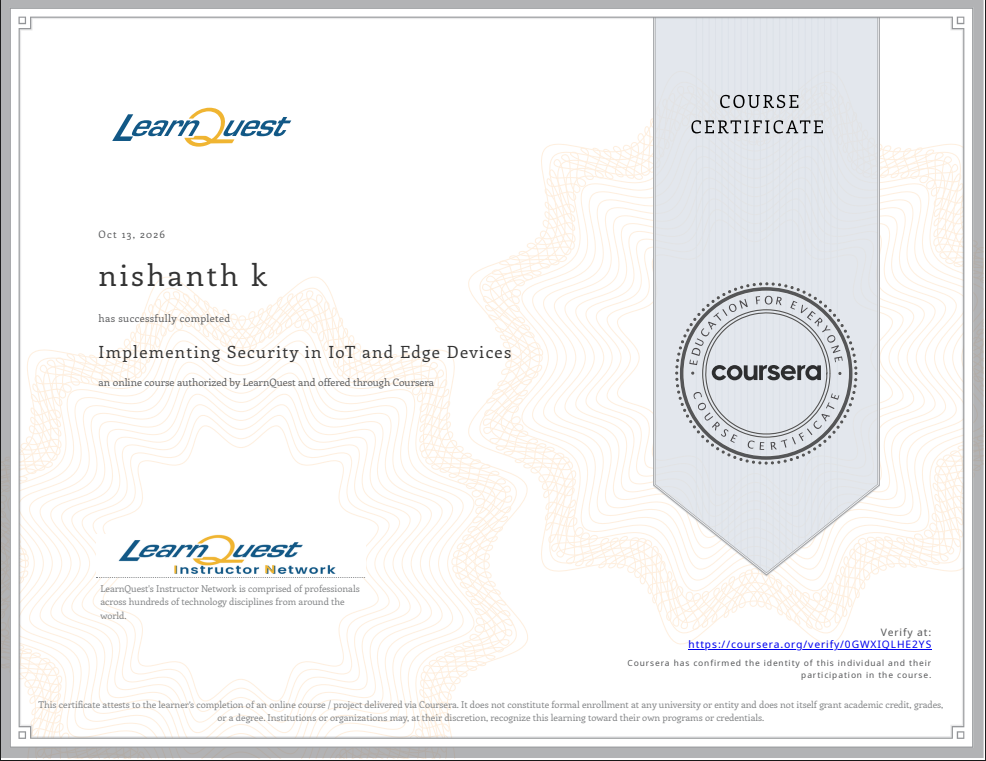
\includegraphics[width=0.96\textwidth, height=0.70\textheight, keepaspectratio]{nishanth_cert.png}}
\end{center}

\vfill
\begin{center}
    {\footnotesize\textbf{Credential Verification URL:} \url{https://coursera.org/verify/0GWXIQLHE2YS}}
\end{center}

\clearpage

% =========================================================
% PAGE 2: TECHNICAL ALIGNMENT REPORT
% =========================================================
\begin{center}
    {\large\textbf{\color{amritablue}AMRITA VISHWA VIDYAPEETHAM}}\\[1pt]
    {\footnotesize\textbf{Amrita School of Computing, Coimbatore --- Department of Computer Science and Engineering}}\\[2pt]
    {\footnotesize\textbf{Technical Enrichment Activity: Professional Online Certification (20 Marks)}}\\[1pt]
    {\scriptsize Course Completion Details \& One-Page Technical Alignment Report}
\end{center}

\vspace{-4pt}
\hrule height 0.8pt
\vspace{4pt}

\noindent
\begin{tabularx}{\textwidth}{@{}l X l X@{}}
    \textbf{Student Name:} & Nishanth K & \textbf{Course Title:} & Implementing Security in IoT and Edge Devices \\
    \textbf{Roll Number:} & CB.SC.U4CSE23523 & \textbf{Platform / Provider:} & Coursera / LearnQuest \\
    \textbf{Degree \& Branch:} & B.Tech CSE (VII Semester) & \textbf{Duration / Effort:} & 12--15 Hours (10--20 Hour Category) \\
    \textbf{Project Guide:} & Ms. Neethu M R (Asst. Professor) & \textbf{Verification URL:} & \url{https://coursera.org/verify/0GWXIQLHE2YS} \\
\end{tabularx}

\vspace{3pt}
\noindent
\textbf{B.Tech Project Title:} \textit{EdgeTrust-VANET: A Decentralized Trust Management and Machine Learning Framework for Secure Vehicular Ad Hoc Networks}

\vspace{2pt}
\section*{1. Course Curriculum \& Technical Competencies Acquired}
The professional certification \textit{Implementing Security in IoT and Edge Devices} (LearnQuest via Coursera) covers formal cyber-physical security principles and defensive engineering for distributed edge ecosystems:
\begin{itemize}
    \item \textbf{Threat Modeling \& Attack Surface Analysis for Edge Nodes:} Analyzing telemetry tampering, sensor spoofing, replay attacks, and denial-of-service vectors at resource-constrained wireless endpoints.
    \item \textbf{Hardware Root of Trust (RoT) \& Cryptographic Key Hygiene:} Embedded cryptographic accelerators, key isolation, secure boot, and evaluating the vulnerabilities of static asymmetric PKI.
    \item \textbf{Edge Anomaly Detection \& Heuristic Firewalls:} Implementing deterministic, low-overhead stream verification to arrest malicious payloads directly at edge compute ingresses.
    \item \textbf{Zero-Trust Architecture \& Dynamic Policy Enforcement:} Continuous behavioral trust evaluation, Bayesian reputation decay, and decentralized certificate revocation mechanisms.
\end{itemize}

\section*{2. Technical Justification: How the Course Directly Supports EdgeTrust-VANET}
Vehicular Ad-hoc Networks (VANETs) represent an extreme class of mission-critical IoT systems characterized by high vehicle speeds (up to 50~m/s), strict 100~ms DSRC beacon deadlines, and resource-constrained automotive microcontrollers. The concepts mastered in this course directly enabled the architectural design and experimental validation of our final year project:

\begin{enumerate}
    \item \textbf{Client-Side Kinematic Heuristic Firewall (Tier 1 --- Vehicle OBUs):} 
    Guided by the course's ingress validation paradigms for sensor endpoints, we formulated an autonomous client-side heuristic firewall ($|a| \le 8.0\,\text{m/s}^2, j \le 10\,\text{m/s}^3$). This filters physically implausible telemetry directly at receiving On-Board Units (OBUs), eliminating \textbf{34.2\% of malicious/redundant wireless transmissions} locally and preventing control channel exhaustion.

    \item \textbf{Embedded Microcontroller Sizing \& Edge ML Predictors (Tier 2 --- Roadside Units):} 
    The course demonstrated that deep neural architectures incur prohibitive latency and memory penalties on edge devices. Applying these profiling principles, we engineered native compiled C++ predictors: Logistic Regression ($0.38\,\mu\text{s}$) and an AdaBoost ensemble with 50 decision stumps ($5.00\,\mu\text{s}$). The resulting binary requires only \textbf{12.4~KB Flash and $<$2~KB RAM}, perfectly matching the L1 cache constraints of automotive safety MCUs (ARM Cortex-R5 / NXP S32G) and complying with ISO 26262 ASIL-D timing deadlines.

    \item \textbf{Overcoming Static PKI Limitations via Behavioral Trust Management:} 
    Standard IEEE 1609.2 PKI verifies sender identity but cannot detect valid keys broadcasting fabricated kinematics. Leveraging the course's behavioral auditing paradigms, we engineered a dynamic dual-dimension trust metric ($T_{\text{final}} = \alpha T_{\text{direct}} + (1-\alpha) T_{\text{indirect}}$, $\alpha^* = 0.65$), cutting the system False Positive Rate by \textbf{85.1\% (down to 1.85\%)} and Malicious Acceptance Rate to \textbf{3.58\%}.

    \item \textbf{Decentralized Fog Consensus \& Rapid Revocation (Tiers 3 \& 4):} 
    The distributed trust management modules directly informed our multi-RSU Beta-Bayesian consensus mechanism ($W = 10\,\text{s}$) and trust-penalized Dijkstra routing, enabling rapid Certificate Revocation List (CRL) propagation without cloud round-trip latency bottlenecks.
\end{enumerate}

\section*{3. Measurable Project Outcomes Supported by this Certification}
\noindent
\begin{tabularx}{\textwidth}{@{}X X X@{}}
    \textbf{Detection Accuracy:} 97.45\% on 15 VeReMi attacks & 
    \textbf{Edge Decision Latency:} 0.38~ms (65$\times$ vs Cloud) & 
    \textbf{Academic Status:} IEEE Conference Paper Under Review \\
\end{tabularx}

\end{document}
